% Chapter 2

\chapter{目标计数方法技术框架}
\section{目标计数}
目前目标计数领域主要有三类方法。一类是检测方法,通过目标检测模型识别出具体的物体位置,之后根据结果来进一步计数。但这类方法对于输入图像的分辨率有着较高的要求,往往需要物体具有明确清晰的边缘特征。在低分辨率下往往表现效果较差。一种是基于回归的方法,直接拟合出图像特征和目标数目之间的回归模型得到图像中对应物体的数目。但这种方法未能完整利用图像中的空间,及序列信息。当输入图像的大小和分布有变化的情况下,往往不具有很强的泛化能力。另一类方法是基于密度图的目标计数方法。此类方法通常先得出一个目标物体在区域内的一个分部,之后就可以通过密度分布来估计总体的数量。该方法在稠密计数的场景下往往具有较好的效果。在本文使用的跨分辨率车辆计数数据集上,可以把车辆计数视为一个稠密计数场景。使用基于密度图的计数方法相较其余两类方法有着更好的表现。
受上述方法启发,本文将跨分辨率车辆计数问题转换为两个子问题,即综合跨分辨率图像信息的图像分割网络和映射分割结果和最终计数目标的回归模型。
\section{语义分割模型}
语义分割作为计算机视觉的一个核心研究方向,目前已经有了较为成熟的解决方法。它的目标是对图像中的每个像素进行细致的分类,从而实现对图像的像素级理解。像素级的输出能力使得该领域的很多方法在密度图的估计上也有着不错的表现。
\subsection{卷积层}
对于图像数据,常使用卷积层而不是全连接层来进行特征提取。卷积层具有的平移不变性和局部性非常适合处理图像数据,可以掌握图像的空间特征。下面给出卷积层的基本定义。
\subsubsection{卷积模型}
\begin{equation}
  \label{eq:eq_conv-layer}
  [\mathbf{H}]{i, j} = u + \sum_{a = -\Delta}^{\Delta} \sum_{b = -\Delta}^{\Delta} [\mathbf{V }]{a, b} [\mathbf{X}]_{i+a, j+b}
\end{equation}
通过使用系数$[\mathbf{V}]{a, b}$对位置$(i, j)$附近的像素$(i+a, j+b)$进行加权得到$[\mathbf{H}]{i, j}$。 其中$|a|> \Delta$或$|b| > \Delta$约束条件使得该式满足局部性,即只关注于在位置像素$(i+a, j+b)$的小领域范围内的参数,大大减少了参数量。$\mathbf{V}$被称为卷积核(convolution kernel)或者滤波器(filter),也是该卷积层的权重,通常该权重是可学习的参数。参数a,b也对应着卷积核的尺寸$k_h,k_w$。
\subsubsection{多通道输入与多通道输出}
上式\eqref{eq:eq_conv-layer}是单通道情况下卷积层的数学表示,当输入图像的通道数为$c_i$时,那么我们需要构造一个形状为$c_i\times k_h\times k_w$的卷积核。由于输入和卷积核都有$c_i$个通道,我们可以对每个通道输入的二维张量和卷积核的二维张量进行互相关运算,再对通道求和得到一个二维张量。这就是一个输出通道的结果。如果我们需要输出通道数为$c_o$时,只需创建一个卷积核的形状是$c_o\times c_i\times k_h\times k_w$。通道数量可以视作对于不同特征的描述,随着神经网络层数的加深,通常的做法是减少空间分辨率的同时增加通道数量。
\subsubsection{填充和步幅}
在应用多层卷积时,我们常常丢失边缘像素。填充(padding)可以解决这个问题。在输入图像的边界填充一定数量的元素(通常填充元素是$0$)。  
通常,如果我们添加$p_h$行填充(大约一半在顶部,一半在底部)和$p_w$列填充(左侧大约一半,右侧一半),则输出形状将为

\begin{equation}
  (n_h-k_h+p_h+1),(n_w-k_w+p_w+1)
\end{equation}
这意味着输出的高度和宽度将分别增加$p_h$和$p_w$。
在许多情况下,我们可以设置$p_h=k_h-1$和$p_w=k_w-1$,这样使得输入和输出具有相同的高度和宽度。假设$k_h$是奇数,我们将在高度的两侧填充$p_h/2$行。 如果$k_h$是偶数,通常会在输入顶部填充$\lceil p_h/2\rceil$行,在底部填充$\lfloor p_h/2\rfloor$行。同理,我们填充宽度的两侧。

感受野是指卷积网络中某一层输出特征图上的一个元素所对应的输入图像上的区域大小。它表征着特征图能“看到”的区域的大小。我们可以通过连续的卷积来增加感受野,但这会增加参数量。我们还可以通过调整步幅来增大感受野。
步幅是卷积操作中卷积核移动的步长。在对图像进行卷积时,卷积核从图像的一个角落开始,按照指定的步幅在图像上滑动,每次移动指定的像素数,直到覆盖整个图像。当步幅大于1时,卷积核每次移动多个像素,输出的特征图的尺寸也会随之减小。具体公式如下:

通常,当垂直步幅为$s_h$,水平步幅为$s_w$时,输出形状为
\begin{equation}
  \lfloor(n_h-k_h+p_h+s_h)/s_h\rfloor \times \lfloor(n_w-k_w+p_w+s_w)/s_w\rfloor
\end{equation}
如果我们设置了$p_h=k_h-1$和$p_w=k_w-1$,则输出形状将简化为$\lfloor(n_h+s_h-1)/s_h\rfloor \times \lfloor(n_w+s_w-1)/s_w\rfloor$。 更进一步,如果输入的高度和宽度可以被垂直和水平步幅整除,则输出形状将为$(n_h/s_h) \times (n_w/s_w)$。
\subsection{激活函数}
卷积神经网络中常用的激活函数包括ReLU(线性整流单元)、Sigmoid、Tanh(双曲正切)等。这些激活函数的目的是在网络中引入非线性特性,使得网络能够学习到更加复杂的数据表示。本文用到的是 线性整流函数ReLU (Rectified Linear Unit)函数和Sigmoid函数。
对于给定元素$x$,ReLU函数被定义为该元素与$0$的最大值。它是目前最常用的激活函数之一。因为它的导数在大于0时为1,小于0时为0,这使得它可以用来缓解梯度消失的问题。
\begin{equation}
  f(x) = \max(0, x)
\end{equation}

Sigmoid函数将输入值映射到(0, 1)区间,这常常用于分类预测或者给出概率预测。然而,由于其在输入值绝对值较大时梯度接近0,可能会导致梯度消失问题。
\begin{equation}
  f(x) = \frac{1}{1 + e^{-x}}
\end{equation}

\subsection{池化层}
池化(pooling)是卷积神经网络中常见的一种方法,主要用于减少特征图的维度,减少计算量的同时保留重要的一致性信息。与卷积层类似,池化运算也是通过一个固定形状的窗口滑动来实现的。与之不同的是,池化通过对邻近像素进行统计学操作(如取最大值或平均值)来实现,因此也不包含参数。主要有两种类型的池化:最大池化(Max Pooling)和平均池化(Average Pooling)。
池化操作通常有两个参数:池化核的大小(KxK)和步幅(S)。池化核指定了池化操作的邻域范围,步幅定义了池化操作的移动间隔。对于输入大小为$W \times H$的特征图,池化操作后的输出大小$W' \times H'$可以通过以下公式计算:
\begin{equation}
  W' = \left\lfloor\frac{W - K}{S} + 1\right\rfloor
\end{equation}
\begin{equation}
  H' = \left\lfloor\frac{H - K}{S} + 1\right\rfloor
\end{equation}

在卷积网络的实践中,池化层通常有降低特征维度、引入不变性、增加鲁棒性和防止过拟合的作用。

\subsection{权重衰减}
在模型训练时,可能会遇到过拟合的问题,使得模型在已有数据上有着较好的性能,而在测试数据上表现不佳。我们可以使用多种正则化技术来缓解过拟合的问题。权重衰减(weight decay)是最广泛使用的正则化的技术之一, 它通常也被称为$L_2$正则化。
$L_2$ 正则化在损失函数中添加模型权重的平方之和作为惩罚项。同时通过一个非负的超参数$\lambda$来控制正则化的强度。$L_2$正则化正则化修正后的损失函数如下式:
\begin{equation}
  L(\mathbf{w}, b)=\frac{1}{n} \sum_{i=1}^{n} \frac{1}{2}\left(\mathbf{w}^{\top} \mathbf{x}^{(i)}+b-y^{(i)}\right)^{2}+\frac{\lambda}{2}\|\mathbf{w}\|^{2}
\end{equation}

L2正则化的目的是鼓励模型学习到更小更分散的权重值,从而提高模型的泛化能力。它对大的权重值施加较大的惩罚,从而防止模型依赖于少数几个可能具有高噪声的特征。

\subsection{暂退法}
Dropout在训练过程中以一定几率随机“丢弃”(即暂时移除)网络中的一部分神经元(包括其连接),这有助于模型学习到更加鲁棒的特征,减少神经元间复杂的共适应关系。需要注意的是,在测试时,我们通常不使用dropout。
\subsection{批量归一化}
批量归一化(Batch Normalization)是通过对每个小批量数据进行归一化处理,调整神经网络中间层的输出,使其均值接近0,标准差接近1。这可以通过减去它们的均值除以它们的标准差得到。这有助于稳定和加速深度网络的训练过程,同时也具有一定的正则化效果。
批量归一化(Batch Normalization,简称BN)是一种在深度神经网络中广泛使用的技术,用于加速训练过程并提高模型的稳定性。其基本思想是在网络的每层之后添加一个归一化步骤,这个步骤会对每个小批量数据(mini-batch)进行归一化处理,以确保网络中间层的激活分布保持稳定。批量归一化的公式如下:

\begin{equation}
  \hat{x}_i = \frac{x_i - \mu_B}{\sqrt{\sigma_B^2 + \epsilon}} 
\end{equation}
其中,$\epsilon$是一个很小的数,用来防止除以零。归一化后的\(\hat{x}_i\)具有零均值和单位方差。

\section{U-Net网络}
U-Net
\cite{ronnebergerUNetConvolutionalNetworks2015}是一个广泛被应用的语义分割模型,最初被应用于医学图像的分割问题上。U-Net是一个具有对称结构的网络,通过使用跳跃连接(Skip Connection)来结合低层次的位置信息和高层次的语义信息,从而在细节上进行更准确的预测。
\begin{figure}[h]
  \centering
  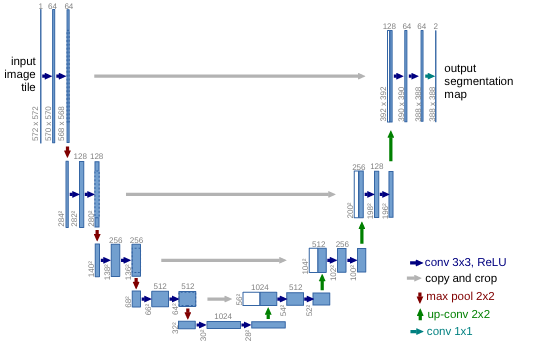
\includegraphics[width=\textwidth]{Unet.png}
  \caption{U-Net网络结构}
  \label{fig:UNet}
\end{figure}
\subsection{模型结构}
U-Net网络由一个收缩路径(contracting path)和一个扩展路径(expansive path)组成.网络的输入是一张$572\times 572$的的图片(input image tile)。网络最终的输出为同样尺寸的分割图预测。图像经过收缩路径提取综合特征,并保留中间特征信息。在扩展路径中,综合上采样后前一层特征结果与对应尺度的编码特征 ,得到最终的结果。因为整个网络结构形似字母‘U’,因此称为U-Net。
\subsection{收缩路径}
收缩路径是由多个卷积层、线性整流函数单元(ReLU)和最大汇聚层(Max Pooling)构成的一系列降采样操作。论文中将这一部分叫做压缩路径(contracting path)。压缩路径由4个块组成,每个块使用了3个有效卷积和1个Max Pooling进行下采样。每个块处理之后特征图的通道数扩大为2倍,特征图的长和宽也有相应缩小。这样的处理使得不同的特征被逐步提取到不同的通道中。最终得到了尺寸为$32\times 32$的特征图。
\subsection{扩展路径}
扩展路径是相同数量的相似模块组成。不同的是扩展路径中使用了反向卷积和上采样。同时扩展路径通过跳跃连接从收缩路径对应的层中获取特征图,并与当前层的特征图进行融合。这种结构有助于恢复图像的精细信息,使得在深度网络中消失的某些信息不至被遗忘。
在深度学习和计算机视觉中,上采样(Upsampling)和反向卷积(也称为转置卷积,Transposed Convolution)是两种常用的技术,用于增加图像或特征图的分辨率。这两种技术常见于像U-Net这样的网络结构中,用于从深层特征映射中恢复图像的细节信息,尤其在图像分割和生成模型中十分重要。

\subsection{双线性插值}
上采样是一种用于增加图像或特征图的尺寸的方法。它通过已有数据的插值来增加分辨率,主要有最近邻插值、双线性插值和双三次插值等方法。下面主要介绍双线性插值。
在双线性插值中,输出像素的值是输入像素值的加权平均,权重基于像素之间的距离。假如我们想得到未知函数 f 在点 $P=\left( x, y\right)$ 的值,假设我们已知函数 f 在 $Q_{11} = \left( x_1, y_1 \right) $, $Q_{12} = \left( x_1, y_2 \right) $, $Q_{21} = \left( x_2, y_1 \right) $, 及 $Q_{22} = \left( x_2, y_2 \right) $ 四个点的值。 

首先在 x 方向进行线性插值,得到:
\begin{align}
f(x, y_1) &\approx \frac{x_2-x}{x_2-x_1} f(Q_{11}) + \frac{x-x_1}{x_2-x_1} f(Q_{21}), \\
f(x, y_2) &\approx \frac{x_2-x}{x_2-x_1} f(Q_{12}) + \frac{x-x_1}{x_2-x_1} f(Q_{22}).
\end{align}

然后在 y 方向进行线性插值,得到 
\begin{equation}
  \begin{aligned}
    f(x,y) &\approx \frac{y_2-y}{y_2-y_1} f(x, y_1) + \frac{y-y_1}{y_2-y_1} f(x, y_2) \\
&= \frac{y_2-y}{y_2-y_1} \left ( \frac{x_2-x}{x_2-x_1} f(Q_{11}) + \frac{x-x_1}{x_2-x_1} f(Q_{21}) \right ) \\
&+ \frac{y-y_1}{y_2-y_1} \left ( \frac{x_2-x}{x_2-x_1} f(Q_{12}) + \frac{x-x_1}{x_2-x_1} f(Q_{22}) \right ) \\
&= \frac{1}{(x_2-x_1)(y_2-y_1)} \big( f(Q_{11})(x_2-x)(y_2-y)+ f(Q_{21})(x-x_1)(y_2-y)\\
&+  f(Q_{12})(x_2-x)(y-y_1) + f(Q_{22})(x-x_1)(y-y_1) \big)\\
&=\frac{1}{(x_2-x_1)(y_2-y_1)}  \begin{bmatrix} x_2-x & x-x_1 \end{bmatrix} \begin{bmatrix} f(Q_{11}) & f(Q_{12}) \\ f(Q_{21})& f(Q_{22}) \end{bmatrix} \begin{bmatrix}
y_2-y \\ y-y_1 \end{bmatrix}.
  \end{aligned}
\end{equation}

如果先在 y 方向插值、再在 x 方向插值,其结果与按照上述顺序双线性插值的结果是一样的。由上式我们不难看出,双线性插值由两个线性函数的积构成,因此为网络带来了非线性。

\subsection{转置卷积}

转置卷积\cite{2018guideconvolutionarithmeticdeeplearning}是一种更复杂的上采样技术,它通过神经网络来试图学习一种更有效的插值方式。它不仅增加了特征图的尺寸,还可以学习在上采样过程中引入新的信息。它通过反转卷积操作的流程实现,因此被称为转置卷积。
标准卷积操作是将卷积核应用于多个输入上,得到一个输出,实际上就是建立了一个多对一的关系。对于转置卷积而言,我们实际上是想建立一个逆向操作,也就是建立一个一对多的关系。对于标准卷积,我们有:
\begin{equation}
𝑌=𝐶𝑋
\end{equation}

转置卷积其实就是要对其进行逆操作,求出X
\begin{equation}
  X=C^T Y
\end{equation}
假设输入特征图大小为\(W \times H\),卷积核大小为\(K \times K\),步长为\(S\),填充为\(P\),输出特征图大小可以通过以下公式计算:

\[ W' = S(W-1) + K - 2P \]
\[ H' = S(H-1) + K - 2P \]

这里\(W'\)和\(H'\)分别是输出特征图的宽度和高度。

\section{注意力机制}
注意力机制(Attention Mechanism)是一种模仿认知注意力的机制。在认知科学中,由于信息处理的瓶颈,人类会选择性地关注信息中的某一一部分,同时忽略其他可见的信息。上述机制通常被称为注意力机制。随着该机制在Transformer、BERT、GPT等NLP领域的成功,该机制及应用又成为了研究的热点话题。目前在计算机视觉领域,ViT、Flow1D等网络也都基于注意力机制进行设计。
从注意力的形式来分类的话,可以分为软注意力(soft attention)和硬注意力(hard attention)。其中软注意力机制是可微可导的,本文中主要探讨的也是软注意力机制。

\subsection{注意力机制基本原理}

\begin{figure}[h]
  \centering
  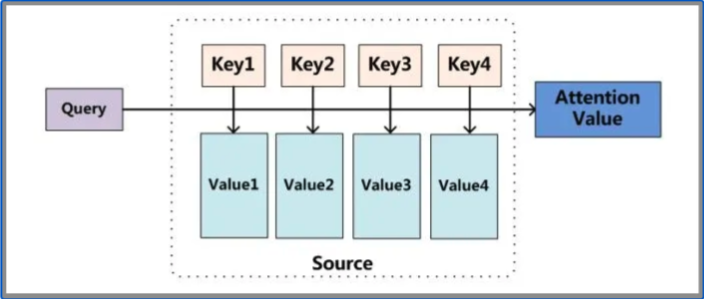
\includegraphics[width=\textwidth]{attention.png}
  \caption{注意力机制}
  \label{fig:attention}
\end{figure}

如图~\ref{fig:attention}所示,注意力机制主要涉及到3类数据,分别是键(key)、值(value)和查询(query)。当一个查询值到来时,计算查询和键的相似度,得到权重,并进行归一化处理。再将得到的权重和值加权求和得到我们最终的注意力结果。
首先计算查询与每个键之间的相似度。这一步通常使用点积(dot product)或者缩放点积(scaled dot product)来实现。具体来说,对于每个查询,通过计算它与所有键的点积,得到一个相似度分数:
\begin{equation}
  \text{score}(Q, K) = QK^T 
\end{equation}

接下来使用Softmax函数对上一步得到的相似度分数进行归一化,以确保所有的权重加起来等于1。:
\begin{equation}
   \text{Attention Weight} = \text{Softmax}(\text{score}(Q, K))
\end{equation}

用归一化后的权重对值进行加权求和,得到最终的注意力输出:
\begin{equation}
  \text{Output} = \text{Attention Weight} \cdot V 
\end{equation}

将上述步骤合并,注意力机制的输出可以通过以下公式计算:
\begin{equation}
\text{Attention}(Q, K, V) = \text{Softmax}\left(\frac{QK^T}{\sqrt{d_k}}\right)V 
\end{equation}

其中,\(d_k\)是键的维度,这个因子用于缩放点积,避免在维度很高时计算结果过大,导致Softmax函数处于饱和区,从而缓解梯度消失的问题\cite{2023AttentionAllYouNeed}。
\subsection{注意力机制在图像领域的应用}
在图像处理领域中,使用注意力机制可以显著提升模型的性能,尤其是在图像分类、目标检测和图像分割等任务中。根据任务需要不同,常用的注意力机制有以下几种:
\begin{enumerate}    
  \item 空间注意力(Spatial Attention):关注图像的特定区域,通常用于增强模型对图像中重要部分的感知能力。可以用来替代传统的卷积网络,找到目标区域。
  \item 通道注意力(Channel Attention):关注不同通道的相关性,可以帮助模型识别哪些特征是更加重要的。
  \item 自注意力(Self-Attention):通过计算图像内所有位置之间的关系,可以捕捉更广泛的上下文信息。在时间序列模型中,自注意力机制可以保证长序列中的所有位置的信息有参与后续计算的可能。在图像领域中,对图像数据自身使用自注意力机制使得输出中每一位置均含有输入图像中所有位置的加权信息。
\end{enumerate}

在图像领域实践中,同时还使用以下几种训练策略:
\begin{enumerate}    
  \item 多尺度注意力:使用多尺度注意力可以帮助模型同时关注图像的粗略和详细特征,这在处理具有不同尺寸和形状的对象时特别有效。
  \item 融合不同的注意力机制:同时使用空间和通道注意力,或者将传统的注意力机制与自注意力结合起来,可以提取更丰富的特征并提高模型的性能。
  \item 注意力正则化:添加注意力正则化可以防止模型对某些特征过度依赖,从而提高模型的泛化能力。使用如残差连接等设计可以训练更深层的网络,防止训练过程中的信息丢失。
\end{enumerate}

\subsection{注意力机制处理序列图像}
在处理序列图像,如视频帧、时间序列的医学图像或连续的监控遥感数据时,我们不仅要考虑图像中的空间信息,也需要考虑图像间的序列信息。对于注意力机制的设计使用有着更高的要求。自注意力机制和多图像帧的相互注意力机制常常用来捕获时间和空间上的复杂关系。以下是这些注意力机制在序列图像处理中的一些常见应用方式:

自注意力机制可以用于分析序列图像中的时间依赖性,这对于识别视频中的动态事件或时间序列图像中的变化特别有效。
\begin{enumerate}    
  \item 时间自注意力:在处理视频或其他序列图像时,可以在时间维度上应用自注意力,以识别不同时间点图像帧之间的关键依赖关系。在视频帧序列中,模型可以学习到哪些帧之间具有高度相关性,这对于动作识别、事件检测等任务非常有用。
  \item 空间自注意力:在单个图像帧内部,可以应用空间自注意力来分析图像中不同区域之间的相互作用,对于解决目标检测和图像分割等任务有很大的帮助。
  \item 时空自注意力:结合时间和空间自注意力,可以同时考虑空间位置和时间演变的关系。这种方法可以用于复杂场景的动态解析,如多物体交互的场景。
\end{enumerate}
 这些方法在处理动态场景解析和增强特征表示上有着不错的表现。在动态变化的场景中,模型可以使用多目标间的相互注意力来预测未来的状态。而通过计算不同目标之间的相互关系,可以获得更丰富的场景表示,这对于场景分类、事件检测等任务非常有帮助。


\section{Attention U-Net网络}
Attention U-Net是一种结合了注意力机制的UNet网络,最初被应用于医学图像的分割问题上。它在U-Net的架构上增加了Attention Gate注意力门使得模型能更好的聚焦在目标区域。
\begin{figure}[h]
  \centering
  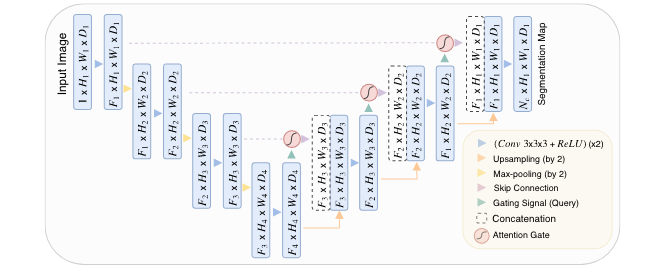
\includegraphics[width=\textwidth]{attention Unet.png}
  \caption{Attention U-Net}
  \label{fig:attentionunet}
\end{figure}

如图~\ref{fig:attentionunet}所示,Attention U-Net沿用了U-Net的基本架构,包括编码器(逐步下采样)和解码器(逐步上采样)两部分,以及跳跃连接(skip connections)来保留多尺度的特征。值得注意的是在每个跳跃连接处,新引入了注意力门控模块。这些模块对来自编码器的特征图进和解码器的相应特征图进行注意力计算。这使得网络能够聚焦于那些对最终分割任务更为重要的区域。

该方法将来自解码器的特征图作为查询,将来自编码器的特征图作为值和键作为注意力门的输入。注意力系数是通过一个小型的卷积网络学习到的,该网络计算当前解码器特征和对应编码器特征之间的相关性。
\begin{figure}[h]
  \centering
  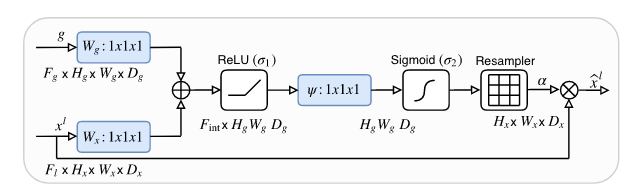
\includegraphics[width=\textwidth]{attention gate.png}
  \caption{Attention gate}
  \label{fig:attentiongate}
\end{figure}


在图~\ref{fig:attentiongate}中展示的是一个注意力门结构。注意力门接收两组输入,一组是来自上一下采样层的特征图(\(g\)),作为查询。另一组是来自跳跃连接的特征图(\(x^l\))键和值。
两组特征图首先通过一个\(1 \times 1 \times 1\)的卷积层(表示为\(W_g\)和\(W_x\)),这一步用于减少通道的数量,以降低后续计算复杂度。
接着,两组卷积后的特征图相加,并通过ReLU激活函数,得到\( \sigma_1\)。经过ReLU激活的特征图再次经过一个\(1 \times 1 \times 1\)卷积层,通常标识为\(\psi\),然后通过Sigmoid激活函数得到\( \sigma_2\),此时每个特征的激活值位于[0, 1]区间,代表了特征的重要性权重。将Sigmoid输出的权重与跳跃连接的特征图(\(x^l\))相乘。在这个过程中,三个\(1 \times 1 \times 1\)卷积层包含了我们需要学习的参数,也赋予了该模块掌握关键权重的能力。通过注意力门,我们得到了在解码器特征图做查询的情况下的加权编码器特征图。利用我们新得到的特征图来进行下一步解码,比原本单纯接受编码器输入获得了更丰富的信息。

\section{Flow1D网络}
Flow1D网络是一个基于注意力机制的光流估计网络。光流估计是计算机视觉中的一个基本问题,它旨在估计一幅图像上的每个像素点在时间序列中的运动,这在视频处理、运动分析、超分辨率、3D重建和自动驾驶等众多领域中都有广泛应用。光流估计是计算机视觉领域中的一个核心问题,光流是图像中像素点在时间维度上的瞬时运动速度和方向的场。光流是从连续的视频帧中估计出来的,这些连续的图像不仅具有时间上的连续性,光流也是从这些图像的空间关系中估计出来的。本文探讨的跨分辨率车辆计数问题,需要从同一时间的高分辨率低分辨率图像中找到空间一致性的关联,同时在连续的低分辨率图像中也要找到时间上的连续性关系。这和光流估计对于连续图像数据的利用有着不少相同之处。

\begin{figure}[h]
  \centering
  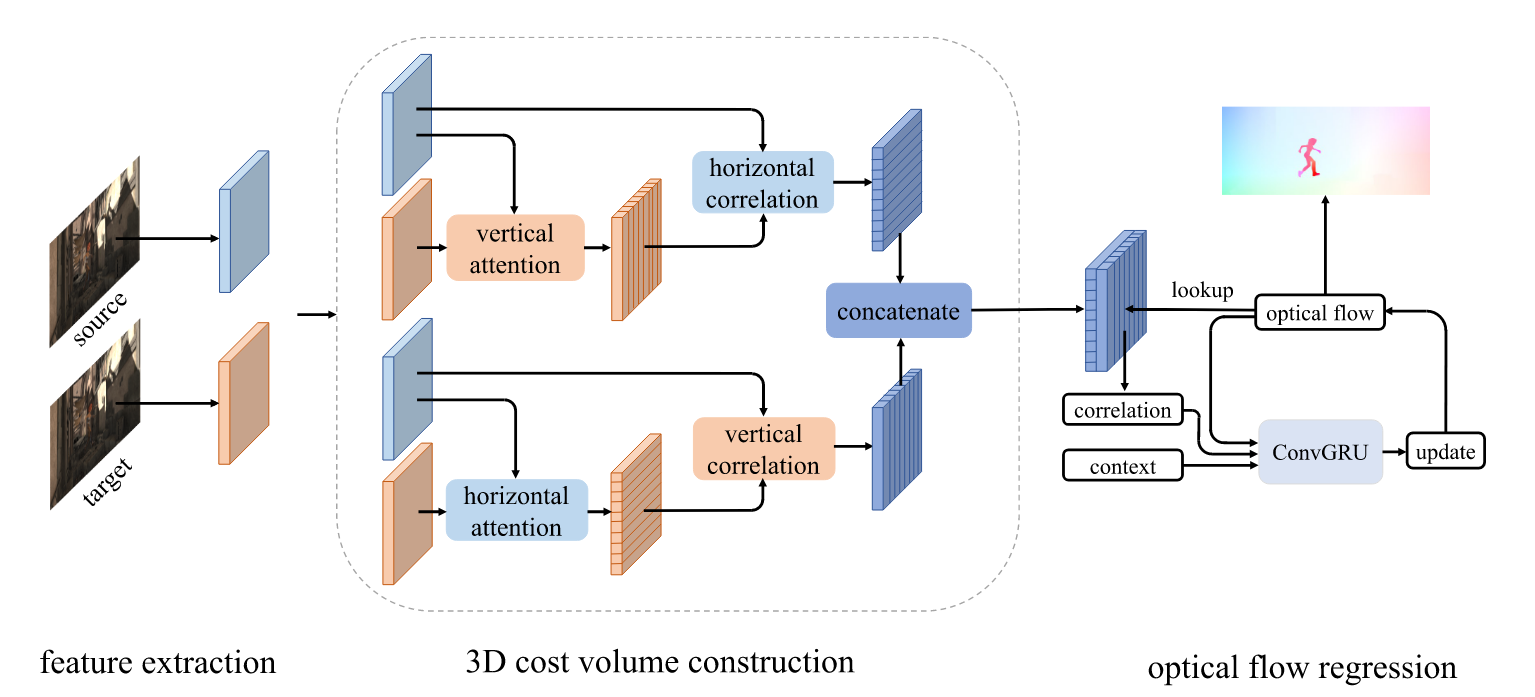
\includegraphics[width=\textwidth]{flow1d.png}
  \caption{Flow1D网络}
  \label{fig:Flow1D}
\end{figure}

上图~\ref{fig:Flow1D}展示了模型的基本框架。对于源和目标两个图像,先分别进行特征提取,然后利用注意力机制计算3D cost volume。最后通过门控循环单元,通过相关性特征和初始提取出的特征,进行隐状态的计算。反复迭代计算出光流。
其中3D cost volume的设计充分利用了注意力机制的全局观察能力,通过两个一维的注意力操作,表征三维的光流状态。在水平竖直方向分别进行自注意力计算和相互之间的注意力计算。

\begin{figure}[h]
  \centering
  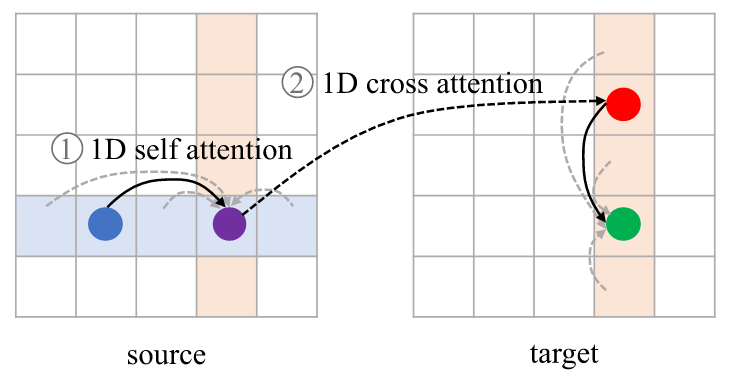
\includegraphics[width=\textwidth]{selfcross.png}
  \caption{self attention和cross attention}
  \label{fig:selfcross}
\end{figure}

图~\ref{fig:selfcross}是一个很直观的展示。如果要计算源和目标的相关度,直接进行cross attention是不能得到红点与蓝点之间的相关关系的。因此需要再源上先进行self attention,使得每一个列向量包含着原先该列的一种加权分布。然后再进行cross attention操作,综合不同图像不同位置的信息。这是一种非常有效的策略。



